\appendix

\section{Experimental Details}
\label{appx:exp}

\subsection{Dataset.}
\label{appx:data}
We conduct experiments on three large-scale traffic datasets: San Diego (SD), Greater Bay Area (GBA), and Greater Los Angeles (GLA) as introduced in the LargeST benchmark~\cite{liu2023largest}. These datasets represent diverse urban settings with varying road network sizes and traffic patterns. 
Additionally, we evaluate on three datasets from different domains: Electricity (ECL), Weather, and ETTh2, where we construct spatio-temporal graphs using node correlation information~\cite{kim2022reversible,wu2021autoformer}.
Following common practice, we chronologically split traffic datasets and ETTh2 into train, validation, and test sets with a ratio of 6:2:2, while using 7:1:2 for ECL and Weather. Sampling frequencies vary across datasets: 5-minute intervals for traffic datasets, 10-minute intervals for Weather, and hourly intervals for ECL and ETTh2.
Table~\ref{tab:dataset} presents detailed statistics of these datasets.
\begin{table}[!ht]
\centering
\scalebox{0.7}{
\begin{tabular}{c|c|c|c|c|c}
\toprule[1.5pt]
%\hline
%\rowcolor[gray]{0.85} 
\rowcolor[gray]{0.85} \textbf{Dataset} & \textbf{\# Points} & \textbf{\# Samples} & \textbf{\# TimeSlices} & \textbf{Timespan} & \textbf{Domain} \\
\midrule
GLA & 3,834 & 134M & 35,040 & 01/01/2019-12/31/2019 & Traffic \\
\hline
GBA & 2,352 & 82M & 35,040 & 01/01/2019-12/31/2019 & Traffic \\
\hline
SD & 716 & 25M & 35,040 & 01/01/2019-12/31/2019 & Traffic \\
\hline
ECL & 321 & 8.4M & 26,304 & 01/01/2014-12/31/2014 & Energy \\
\hline
Weather & 21 & 1.1M & 52,696 & 01/01/2020-12/31/2020 & Climate \\
\hline
ETTh2 & 7 & 0.10M & 14,400 & 07/01/2016-06/30/2017 & Energy \\
\hline
\end{tabular}
}
\caption{The Detail of dataset statistics. The graph data for GLA, GBA, and SD are from real-world road networks, while graphs for other datasets are constructed.}
\label{tab:dataset}
\end{table}

\subsection{Baselines.}
\label{appx:baselines}
We compare \model with 1) time-series forecasting models including: \textbf{LSTM}\cite{hochreiter1997long}, a sequence learning approach with gated mechanisms for long-term temporal dependency modeling; \textbf{PatchTST}\cite{nie2022time}, a transformer architecture for long-term forecasting, showing strong performance through its patch-based approach; \textbf{iTransformer}\cite{liu2023itransformer}, an inverted transformer method that treats every variate as a token, applies self-attention to capture cross-variate correlations;
\textbf{DLinear}\cite{zeng2023transformers}, a linear transformation approach simplifying the prediction process under the assumption of linear changes over time;
and 2) spatio-temporal forecasting methods including: 
\textbf{DCRNN}\cite{li2017diffusion}, integrating diffusion convolution with RNNs using bidirectional random walks;
\textbf{STGCN}\cite{yu2017spatio}, combining graph convolutions with gated temporal convolutions for efficient spatio-temporal feature extraction;
\textbf{ASTGCN}\cite{guo2019attention}, employing spatio-temporal attention mechanisms for dynamic feature weighting;
\textbf{STTN}\cite{xu2020spatial}, a transformer-based approach capturing global dependencies through multi-head self-attention mechanisms;
\textbf{AGCRN}\cite{bai2020adaptive}, learning node-specific patterns through adaptive graph convolutions with parameter-efficient node embeddings;
\textbf{STGODE}\cite{fang2021spatial}, modeling continuous dynamics with neural ODEs to better approximate the underlying physical processes;
\textbf{DGCRN}\cite{li2023dynamic}, adapting to evolving traffic patterns with dynamic graph convolutions and recurrent state updates;
\textbf{D2STGNN}\cite{shao2022decoupled}, decoupling spatio-temporal dependencies for efficient representation;
\textbf{DSTAGNN}\cite{lan2022dstagnn}, leveraging dynamic spatio-temporal attention for capturing complex dependencies;
\textbf{STWave}\cite{fang2023spatio}, using wavelet transforms to capture multi-resolution traffic patterns in both spatial and temporal domains; and
\textbf{BigST}\cite{han2024bigst}, a distributed framework optimized for large-scale ST data processing with memory-efficient implementations.

\subsection{Evaluation Metrics.}
\label{appx:metrics}
To evaluate forecasting performance, we adopt three widely-used metrics: Mean Absolute Error (MAE), Root Mean Square Error (RMSE), and Mean Absolute Percentage Error (MAPE) defined as follows. These metrics are calculated across different prediction horizons (3, 6, and 12 steps ahead) and their averages to comprehensively assess prediction accuracy at various time steps.
\begin{align}
\mathrm{MAE}&=\frac{1}{|\mathcal{V}|}\sum_{(b,t,n)}|y-\hat{y}|,\\
\mathrm{RMSE}&=\sqrt{\frac{1}{|\mathcal{V}|}\sum_{(b,t,n)}(y-\hat{y})^{2}},\\
\mathrm{MAPE}&=\frac{100}{|\mathcal{V}|}\sum_{(b,t,n)}\frac{|y-\hat{y}|}{y+\epsilon},
\end{align}
where $\mathcal{V}$ is the set of valid (non-missing) entries and $\epsilon=10^{-5}$ prevents division-by-zero.

\subsection{Optimization Settings.}
\label{appx:optim}
Our framework is implemented in PyTorch and trained on an NVIDIA A6000 GPU (48GB). We use the Adam optimizer with an initial learning rate of 0.001 and a weight decay of 0.0001. The batch size is set to 8 for GLA, 16 for GBA, and 64 for others (reduced by half if OOM occurs). All models are trained for a maximum of 300 epochs with early stopping (patience of 10 epochs) to prevent overfitting. For fair comparisons, all baseline models are implemented with their recommended configurations, as referred to in BasicTS~\cite{shao2024exploring}, and optimized separately for each dataset. All transformed visual modalities have a resolution of 128×128 pixels with 3 channels.

% \section{Visualization of Constructed Matrix}
% % \label{appx:matrix}
% % \begin{figure}[h]
% % \centering
% % \includegraphics[width=.9\linewidth]{fig/correlation_heatmap.pdf}
% % \caption{Example correlation matrices (left) and block-wise attention weights (right) on GLA.}
% % \end{figure}

% \section{Contribution of Each Modality}
% \label{appx:modality}
% \begin{table}[h]
% \centering\small
% \caption{Ablation on modality contribution (12-step horizon, SD).}
% \begin{tabular}{lccc}
% \toprule
% Variant & MAE $\downarrow$ & RMSE $\downarrow$ & MAPE\% $\downarrow$\\
% \midrule
% Full ViST & \textbf{21.21} & \textbf{36.23} & \textbf{13.86}\\
% w/o Vision & 54.34 & 77.43 & 70.17\\
% w/o Text   & 26.76 & 44.09 & 17.20\\
% w/o Graph  & 24.86 & 41.59 & 17.84\\
% \bottomrule
% \end{tabular}
% \end{table}

% \section{Efficiency Analysis}
% \begin{table}[!ht]
\centering
\small
%\renewcommand{\arraystretch}{1.2}
\resizebox{1.0\linewidth}{!}{
\begin{tabular}{l|cccc|cccc}
\toprule[1.0pt]
\textbf{Dataset} & \multicolumn{4}{c|}{\textbf{GBA}} & \multicolumn{4}{c}{\textbf{GLA}} \\
\hline
\textbf{Methods} & \textbf{BS} & \textbf{Mem} & \textbf{Train} & \textbf{Val} & \textbf{BS} & \textbf{Mem} & \textbf{Train} & \textbf{Val} \\
\midrule
\midrule
DCRNN & 16 & 19.51 & 2654.61 & 350.11 & 8 & 30.90 & 6880.55 & 1486.49 \\
DGCRN & 16 & 38.71 & 2834.88 & 809.12 & 4 & 34.90 & 11961.95 & 5332.09 \\
D2STGNN & 4 & 45.10 & 5392.56 & 830.39 & 1 & 16.87 & 24445.55 & 3999.65 \\
STWave & 16 & 24.44 & 982.40 & 152.55 & 8 & 39.54 & 1582.59 & 253.09 \\
ASTGCN & 16 & 4.75 & 1246.94 & 217.51 & 8 & 6.75 & 3639.42 & 648.63 \\
\rowcolor{green!20} {ViST (Ours)} & {16} & 22.26 & {626.58} & {96.27} & {8} & 34.60 & {1227.69} & {176.57} \\
%\rowcolor{green!20} ViST-V & 16 & 22.26 & 626.58 & 96.27 & 8 & 34.60 & 1227.69 & 176.57 \\
%ViST & 16 & 36.55 & 1021.24 & 139.85 & 8 & 45.98 & 2341.48 & 315.00 \\
\hline
\end{tabular}
}
\caption{Memory and efficiency comparisons on two large-scale datasets, GBA (N=2,352) and GLA(N=3,834). BS: the batch size, Mem: CUDA memory (GB) used, Train: training time (seconds per epoch), Val: inference time (in seconds).}
\label{tab:efficiency}
\end{table}

% \model demonstrates strong computational efficiency, as shown in Table~\ref{tab:efficiency}. We selected several models that demonstrated superior performance in previous experiments and evaluated them using the maximum possible batch size on a single GPU, recording memory usage, training time, and inference time. While graph/attention-based models face a quadratic growing computational cost w.r.t. the number of nodes, \model achieves the fastest training and inference speeds across both GBA and GLA datasets, with training times of 626.58 and 1227.69 seconds per epoch respectively, and inference times of 96.27 and 176.57 seconds. While ASTGCN exhibits lower memory consumption, it requires significantly more time for both training and inference, highlighting that our model achieves better resource utilization. Complex models like D2STGNN face severe scalability challenges on large datasets, requiring batch size reduction to 1 for GLA and consuming excessive computation cost.

\section{Justification of  Efficiency}
The scalability of \textbf{ViST} rests on a set of mutually reinforcing design choices that systematically remove the quadratic dependence on the number of nodes~$N$, fundamentally departing from the quadratic dependencies that plague existing graph-based methods.

During the transformation process, the original input tensor $\mathbf{X}\in\mathbb{R}^{T\times N\times D}$ is fully-vectorized by lightweight $3{\times}3$ convolutions and mapped to 3 images of shape $H\times W$ ($H=W\ll N$). The operation costs $\mathcal{O}(THWC)$ and stores only $\mathcal{O}(HWC)$ parameters, both independent of node number $N$. 
This design leverages the inherent sparsity of traffic road networks, where spatial relationships can be effectively captured through compact grid representations. For instance, the largest GLA dataset with $N = 3{,}834$ nodes is effectively encoded on a $64 \times 64$ grid while preserving essential spatial dependencies. This contrasts sharply with graph-based methods like ASTGCN and D2STGNN, which construct attention matrices with $\mathcal{O}(N^2)$ complexity that becomes prohibitive as $N$ scales--evidenced by their out-of-memory failures on large datasets.

The conditional reconstructor operates in a compressed visual space, fusing visual representations $\mathbf{V}$ with structural features $\mathbf{C}_g \in \mathbb{R}^{B \times N \times D_g}$ and textual embeddings $\mathbf{C}_t \in \mathbb{R}^{B \times D_t}$ through multi-scale linear encoders. The computational cost scales as $\mathcal{O}(THW \cdot D_v)$, where the dominant term $THW \cdot D_v \approx 2 \times 10^6$ operations for GLA experiments represents over two orders of magnitude reduction compared to full graph convolutions on all $N$ nodes.

Due to the distributional differences between visual embeddings and hidden embeddings, simply concatenating them and applying multi-head attention not only fails to align modalities effectively but also introduces redundant computational overhead. 
To address this challenge and efficiently fuse cross-modal embeddings while maintaining computational efficiency, we employ dynamic block partitioning for each modality. 
Our BWA mechanism partitions embeddings into $b_t = \lceil L_t^{2/3}\rceil$ and $b_v = \lceil L_v^{2/3}\rceil$ blocks, where $L_t$ and $L_v$ are the sequence lengths of hidden and visual embeddings respectively, reducing cross-attention complexity from $\mathcal{O}(L^2)$ to $\mathcal{O}(b \cdot (L/b)^2)$, where $L$ is the length of $Q,K,V$ and $b$ is the number of blocks. 
By setting $b\approx L^{\frac{2}{3}}$ optimally, we achieve substantial computational savings while maintaining representational capacity.

In practice, \textbf{ViST} requires only 34.6 GB GPU memory and $1{,}227.69$ seconds per training epoch, while competing methods like D2STGNN must reduce batch sizes to $1$ and consume $24{,}445.55$ seconds per epoch. Similarly, ViST achieves the fastest inference times of $96.27$ and $176.57$ seconds on GBA and GLA respectively, establishing its practical deployability at true city scale. These empirical results validate that our framework successfully captures complex spatio-temporal dependencies through visual modality transformation while maintaining computational tractability for large-scale real-world applications.

%\section{Visualization and Interpretability}
\section{Justification of Vision Transformation}

Traditional spatio-temporal forecasting methods encounter fundamental challenges when processing complex multi-dimensional temporal-spatial data: temporal dynamics, spatial relationships, and inter-node dependencies are often handled separately, leading to information fragmentation and computational inefficiencies. Our multi-view vision encoder addresses these limitations by transforming spatio-temporal data into visual representations that enable unified encoding and holistic processing in a low-dimensional space. The underlying methodological innovation lies in leveraging the inherent advantages of visual processing: parallel information encoding capabilities, hierarchical pattern recognition mechanisms, and spatial locality principles.

Our visual embedding is grounded in the essential characteristics and information expression requirements of spatio-temporal data. 
1) The \textbf{TCG} captures sequential evolutionary dynamics through rolling window statistics and exponential decay weighting mechanisms, mapping multi-node temporal patterns into grid-based visual structures that enable convolutional operations to naturally identify periodicity, trends, and anomalous patterns within time series. 
2) The \textbf{SCG} transforms network topological adjacency relationships into visual proximity through feature importance weighting and temporal change enhancement, organically combining spatio-temporal dimensions while preserving spatial connectivity information. 
3) The \textbf{CCG} directly visualizes inter-node correlation matrices as two-dimensional images, revealing latent dependency relationships and dynamic interaction patterns that explicit spatial adjacency cannot capture through sliding window and hidden state fusion mechanisms. This design ensures that the three channels form a complementary information expression system while maintaining their distinctive characteristics.
Our vision transformation approach achieves fully vectorized parallel processing through an initial low-resolution computation followed by a unified upsampling strategy, significantly reducing computational complexity while maintaining representational quality.

To investigate the interpretability of our vision-enhanced approach, we visualize the learned representations from different domains and each image channel using t-SNE, as shown in Figure~\ref{fig:tsne}. The results reveal that our transformed image representations successfully extract essential spatio-temporal features from large-scale traffic data. These visual features are generated from training on the SD dataset and categorized by spatial images (SI), temporal images (TI), and correlation images (CI), demonstrating significant coverage across distributions from various spatio-temporal domains. Specifically, each channel forms distinctive clusters while maintaining connections with others. These clusters not only cover the large-scale training data but also overlap with regions occupied by cross-domain transfer data points from Weather, Electricity, and ETTh2, strongly suggesting the possibility of using visual modality to transfer to vast spatio-temporal scenarios.

The clear pattern separation yet partial overlap between different vision transformation types indicates that all transformation channels and their combination capture complex ST dependencies. These findings not only demonstrate the consistency between ST data and vision transformation in our method but also highlight the potential generalization and transfer capabilities of our framework. The result provides strong evidence that our approach successfully bridges the gap between spatio-temporal data and interpretable visual representations, making complex dynamics more accessible and understandable for multi-modal learning.

\begin{figure}[h]
  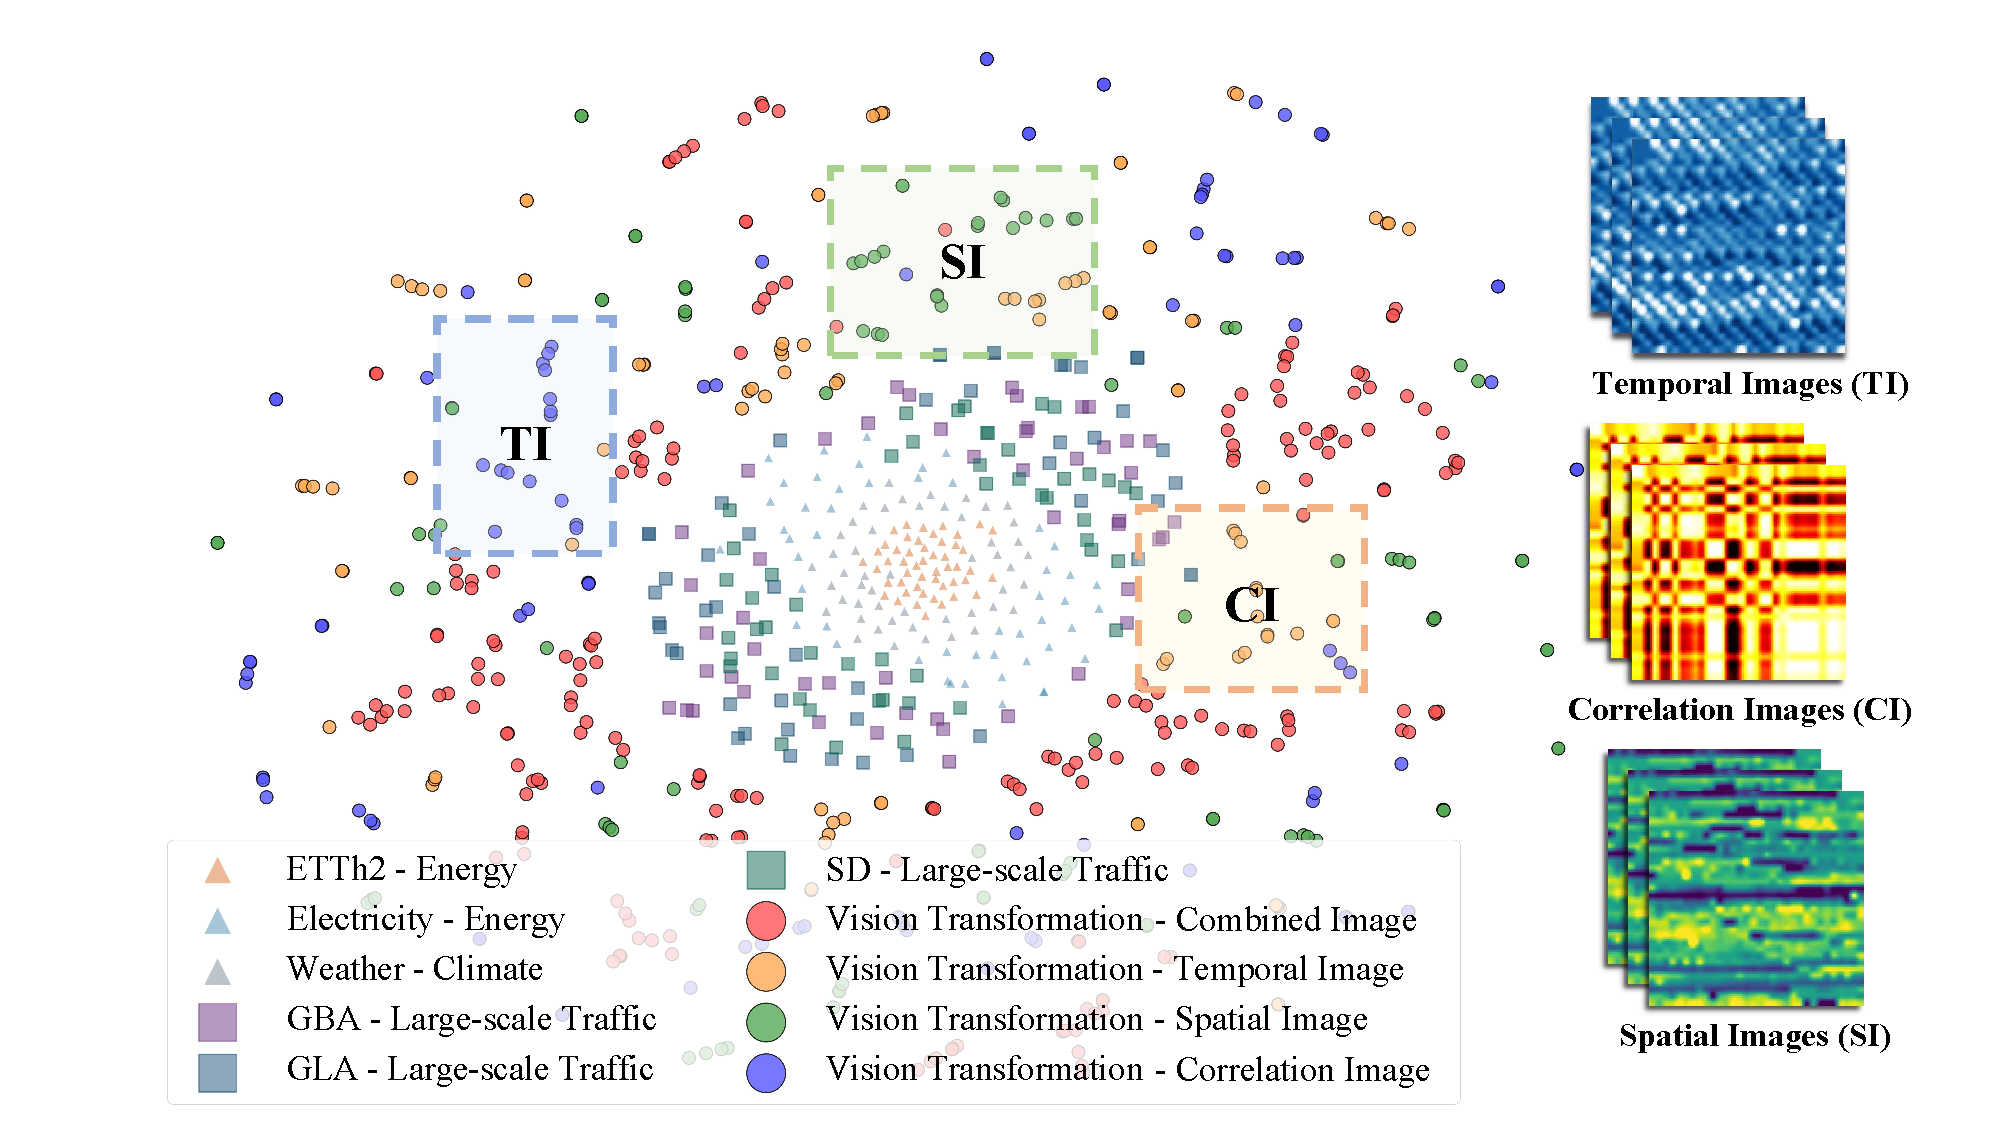
\includegraphics[width=0.48\textwidth]{figures/visualizations.pdf}
  %{figures/tsne_visualization.pdf}
  \caption{The t-SNE visualization of multi-domain data and our transformed visual embeddings. These visual representations cover large-scale traffic data and span other domains like climate and energy with constructed adjacent matrices, validating our approach's capability to reconstruct meaningful visual representations from ST data, and making complex spatio-temporal dependencies more interpretable through the visual modality.}
  \label{fig:tsne}
\end{figure}

\section{Limitation and Future Work}
While \model demonstrates superior performance across multiple domains, several limitations warrant acknowledgment and provide directions for future enhancement. Our current evaluation primarily focuses on established traffic flow, while the framework's generalizability to more complex domains such as epidemic dynamics, urban evolution patterns, or multi-scale environmental monitoring remains to be thoroughly validated. Additionally, the multi-view vision transformation process involves numerous hyperparameters for image processing, which require careful domain-specific tuning despite our comprehensive sensitivity analysis.

In future work, we will explore more effective approaches for transforming spatio-temporal data into visual modality, including learnable transformation functions and masked reconstruction strategies that could enable more adaptive and domain-specific visual representations while leveraging self-supervised learning paradigms. We will investigate the integration of our vision transformation approach with large-scale pre-trained Vision-Language Models (VLMs) such as CLIP, BLIP, and GPT-4V, potentially enabling zero-shot or few-shot adaptation to new spatio-temporal domains by harnessing the rich visual and textual understanding capabilities of these foundation models.

\section{Pseudo Code of ViST}
\label{appx:pseudo}
\begin{algorithm}[H]
\caption{Vision-enhanced Spatio-Temporal Forecasting}
\label{alg:vist}
\begin{algorithmic}[1]
    \REQUIRE Historical observations $\mathbf{X}\!\in\!\mathbb{R}^{B\times T\times N\times D}$,
             adjacency $\mathbf{A}\!\in\!\mathbb R^{N\times N}$,
             description text $\mathcal{D}$
    \ENSURE  Forecast $\widehat{\mathbf{Y}}\!\in\!\mathbb R^{B\times H'\times N\times \mathcal{D}'}$
    \Function{STIM}{\mathbf{X},\mathbf{A}}
        \STATE $\mathbf{E}_{\text{node}}\leftarrow\text{NodeEmbed}(\mathbf{X,A})$
        \STATE $(\mathbf{E}_{\text{tod}},\mathbf{E}_{\text{dow}})\leftarrow\text{TimeEmbed}(\mathbf{X})$
        \STATE $\mathbf{E}_{\text{adp}}\leftarrow\text{Conv}(\mathbf{X})$
        \STATE $\mathbf{H}_t\!\leftarrow\!\text{Conv}\bigl(
               \sigma(\mathbf{E}_{\text{adp}})
               \,\|\,\sigma(\mathbf{E}_{\text{node}})
               \,\|\,\sigma(\mathbf{E}_{\text{tod}})
               \,\|\,\sigma(\mathbf{E}_{\text{dow}})
               \bigr)$
        \RETURN $\mathbf{H_t}$
    %\EndFunction
    \Function{MVE}{\mathbf{H}_t,\mathbf{X},\mathbf{A}}
        % \STATE $\mathbf{V}_s\leftarrow\text{SCG}(\mathbf{X},\mathbf{A})$
        % \STATE $\mathbf{V}_t\leftarrow\text{TCG}(\mathbf{X})$
        % \STATE $\mathbf{V}_c\leftarrow\text{CCG}(\mathbf{X},\mathbf{H}_t,\mathbf{A})$
        %\STATE $\mathbf{V}_s, \mathbf{V}_t, \mathbf{V}_c \leftarrow\text{SCG}(\mathbf{X},\mathbf{A}),\text{TCG}(\mathbf{X}),\text{CCG}(\mathbf{X},\mathbf{H}_t,\mathbf{A})$
        % \STATE $\mathbf{V}\leftarrow[\mathbf{V}_s;\mathbf{V}_t;\mathbf{V}_c]$ % \Comment{concat on channel}
        \STATE $\mathbf{V}\leftarrow [\text{SCG}(\mathbf{X},\mathbf{A});\text{TCG}(\mathbf{X});\text{CCG}(\mathbf{X},\mathbf{H}_t,\mathbf{A})]$
        
        \RETURN $\mathbf{V}$
    %\EndFunction
    \Function{ConditionGeneration}{\mathbf{X},\mathbf{A},\mathcal{D}}
        \STATE $\mathbf{C}_g\leftarrow\text{MultiScaleGraph}(\mathbf{A},\mathbf{X})$
        \STATE $\mathbf{C}_t\leftarrow\text{TextEncoder}(\text{Prompt}(\mathbf{X},\mathcal{D}))$
        \RETURN $(\mathbf{C}_g,\mathbf{C}_t)$
    %\EndFunction
    \Function{CVFR}{\mathbf{V},\mathbf{C}_g,\mathbf{C}_t}
        \STATE $\mathbf{F}_{\text{temp}}\leftarrow\Phi_{\text{temp}}(\mathbf{V})$
        \STATE $\mathbf{F}_{\text{str}}\leftarrow\Phi_{\text{str}}\bigl([\mathbf{F}_{\text{temp}};\mathbf{C}_t]\bigr)$
        \STATE $\mathbf{F}_{\text{text}}\leftarrow\Phi_{\text{text}}\bigl([\mathbf{F}_{\text{str}};\sigma(\mathbf{C}_g)]\bigr)$
        \STATE $\mathbf{H}_v\leftarrow\text{Reshape}\!\bigl(\Phi_{\text{vis}}(\mathbf{V},\mathbf{F}_{\text{text}})\bigr)$
        \RETURN $\mathbf{H}_v$
    %%\EndFunction
    \Function{CrossModalFusion}{\mathbf{H}_t,\mathbf{H}_v}
        \STATE $\{\mathbf{H}_v^{(j)}\}, \{\mathbf{H}_t^{(i)}\} \leftarrow\text{BlockPartition}(\mathbf{H}_v,\mathbf{H}_t)$
        \FORALL{paired blocks $(i,j)$}
            \STATE $\widehat{\mathbf{H}}_t^{(i)}\leftarrow\text{Attention}(
\mathbf{H}_t^{(i)},\mathbf{H}_v^{(j)},\mathbf{H}_v^{(j)})$
            \STATE $\widehat{\mathbf{H}}_v^{(j)}\leftarrow\text{Attention}(                   \mathbf{H}_v^{(j)},\mathbf{H}_t^{(i)},\mathbf{H}_t^{(i)})$
        \ENDFOR
        \STATE $g_t,g_v\leftarrow\text{Softmax}\bigl(\text{MLP}([\widehat{\mathbf{H}}_t;\widehat{\mathbf{H}}_v])\bigr)$
        \STATE $\mathbf{H}_g\leftarrow g_t\!\cdot\!\widehat{\mathbf{H}}_t
                      + g_v\!\cdot\!\widehat{\mathbf{H}}_v$
        \STATE $\mathbf{H}_f\leftarrow\text{FFN}(\text{LayerNorm}(\mathbf{H}_g))+\mathbf{H}_g$
        \RETURN $\mathbf{H}_f$
    %\EndFunction
    \FORALL{mini-batch $(\mathbf{X},\mathbf{A},\mathcal{D},\mathbf{Y})$}
        \STATE $\mathbf{H}_t\leftarrow$\text{STIM}$(\mathbf{X},\mathbf{A})$
        \STATE $\mathbf{V}\leftarrow$\text{MVE}$(\mathbf{H}_t,\mathbf{X},\mathbf{A})$
        \STATE $(\mathbf{C}_g,\mathbf{C}_t)\leftarrow$\text{ConditionGen}$(\mathbf{X},\mathbf{A})$
        \STATE $\mathbf{H}_v\leftarrow$\text{CVFR}$(\mathbf{V},\mathbf{C}_g,\mathbf{C}_t)$
        \STATE $\mathbf{H}_f\leftarrow$\text{CrossModalFusion}$(\mathbf{H}_t,\mathbf{H}_v)$
        \STATE $\widehat{\mathbf{Y}}\leftarrow\text{MLP}(\text{Conv}(\mathbf{H}_f))$
        \STATE $\mathcal L\leftarrow\text{MaskedMAE}(\widehat{\mathbf{Y}},\mathbf{Y})$
        \STATE Update parameters with Adam using $\mathcal L$
    \ENDFOR
\end{algorithmic}
\end{algorithm}

